\documentclass{beamer}
\usepackage{ctex, hyperref}
\usepackage[T1]{fontenc}

% other packages
\usepackage{latexsym,amsmath,xcolor,multicol,booktabs,calligra}
\usepackage{graphicx,pstricks,listings,stackengine}

\author{userElaina}
\title{BPTT}
\subtitle{}
\institute{人工智能学院}
\date{2023.09.02}
\usepackage{JilinUniv}

% defs
\def\cmd#1{\texttt{\color{red}\footnotesize $\backslash$#1}}
\def\env#1{\texttt{\color{blue}\footnotesize #1}}
\definecolor{deepblue}{rgb}{0,0,0.5}
\definecolor{deepred}{rgb}{0.6,0,0}
\definecolor{deepgreen}{rgb}{0,0.5,0}
\definecolor{halfgray}{gray}{0.55}

\lstset{
    basicstyle=\ttfamily\small,
    keywordstyle=\bfseries\color{deepblue},
    emphstyle=\ttfamily\color{deepred},    % Custom highlighting style
    stringstyle=\color{deepgreen},
    numbers=left,
    numberstyle=\small\color{halfgray},
    rulesepcolor=\color{red!20!green!20!blue!20},
    frame=shadowbox,
}


\begin{document}

\kaishu
\begin{frame}
    \titlepage
    \begin{figure}[htpb]
        \begin{center}
            
\includegraphics[width=0.15\linewidth]{pic/Jilin_University_Logo.eps}
        \end{center}
    \end{figure}
\end{frame}

\begin{frame}
    \tableofcontents[sectionstyle=show,subsectionstyle=show/shaded/hide,subsubsectionstyle=show/shaded/hide]
\end{frame}

\section{RNN 的 BPTT 算法}

\begin{frame}
    \begin{figure}[l]
        \centering
        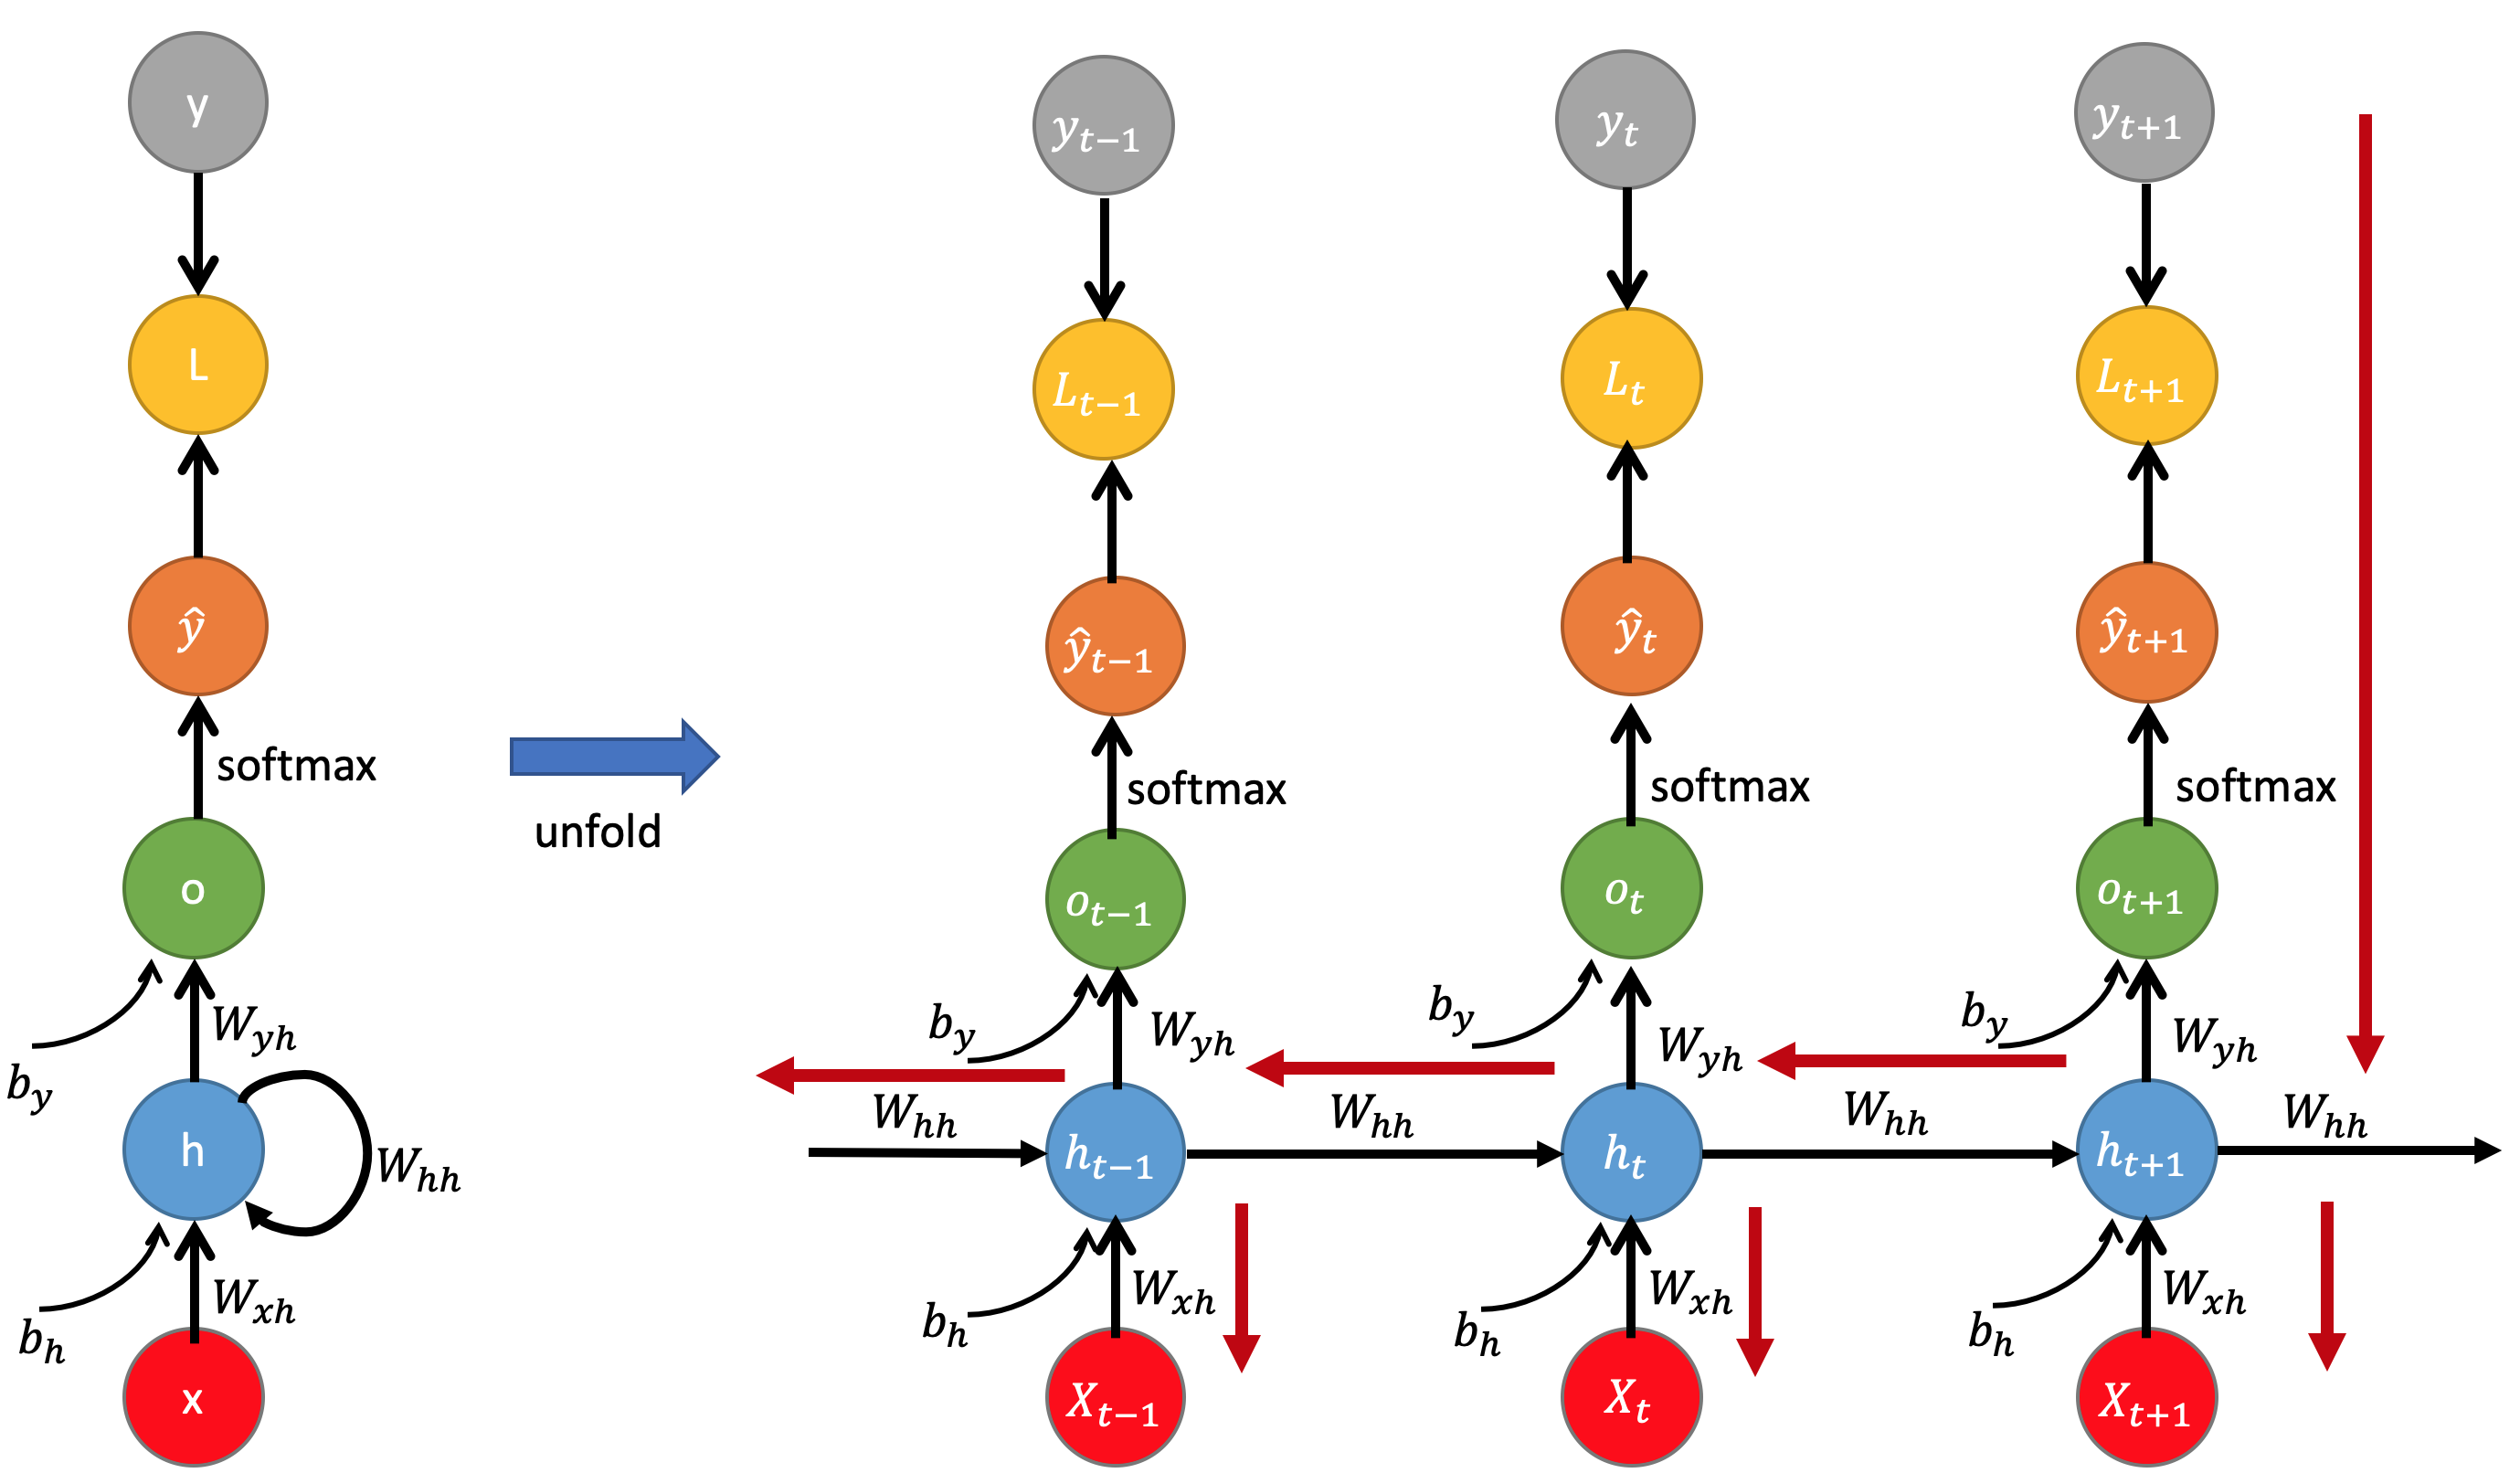
\includegraphics[height=.75\textheight]{pic/bptt.png}
    \end{figure}
\end{frame}

\begin{frame}
    \begin{equation*}
        \begin{aligned}
            h_t &= \Phi_h(X_t\cdot W_{xh}+h_{t−1}\cdot W_{hh}+b_h) \\
            o_t &= h_t\cdot W_{yh}+b_y \\
            \hat{y}_t &= \Phi_o(o_t) \\
            L &= \sum_{i=1}^T L_t \\
            L_t &= -[y_t\log\hat{y}_t+(1-y_t)\log(1-\hat{y}_t)]
        \end{aligned}
    \end{equation*}
\end{frame}

\begin{frame}
    \begin{equation*}
        \begin{aligned}
            \frac{\partial o_t}{\partial W_{yh}}
            &= h_t \\
            \frac{\partial o_t}{\partial h_t}
            &= W_{yh} \\
            \frac{\partial o_t}{\partial b_y}
            &= 1 \\
            \frac{\partial L_t}{\partial\hat{y}_t}
            &= -\frac{y_t}{\hat{y}_t}+\frac{1-y_t}{1-\hat{y}_t} \\
        \end{aligned}
    \end{equation*}
\end{frame}

\begin{frame}
    \begin{equation*}
        \begin{aligned}
            \Phi_o
            &= {\rm softmax} \\
            \frac{\partial\hat{y}_t}{\partial o_t}
            &= \hat{y}_t(1-\hat{y}_t) \\
            \frac{\partial L_t}{\partial o_t}
            &= \frac{\partial L_t}{\partial\hat{y}_t}\frac{\partial\hat{y}_t}{\partial o_t} \\
            &= \hat{y}_t-y_t \\
        \end{aligned}
    \end{equation*}
\end{frame}

\begin{frame}
    \begin{equation*}
        \begin{aligned}
            \frac{\partial L_t}{\partial b_y}
            &= \frac{\partial L_t}{\partial o_t}\frac{\partial o_t}{\partial b_y} \\
            &= \hat{y}_t-y_t \\
            \frac{\partial L_t}{\partial W_{yh}}
            &= \frac{\partial L_t}{\partial o_t}\frac{\partial o_t}{\partial W_{yh}} \\
            &= (\hat{y}_t-y_t)h_t \\
            \frac{\partial L_t}{\partial h_t}
            &= \frac{\partial L_t}{\partial o_t}\frac{\partial o_t}{\partial h_t} \\
            &= (\hat{y}_t-y_t)W_{yh} \\
        \end{aligned}
    \end{equation*}
\end{frame}

\begin{frame}
    \begin{equation*}
        \begin{aligned}
            \frac{\partial L_{t+1}}{\partial W_{hh}}
            &= \frac{\partial L_{t+1}}{\partial h_{t+1}}\frac{\partial h_{t+1}}{\partial W_{hh}} \\
            &= \frac{\partial L_{t+1}}{\partial h_{t+1}}\frac{\partial h_{t+1}}{\partial h_t}\frac{\partial h_t}{\partial W_{hh}} \\
            &= \sum_{k=1}^{t+1}\frac{\partial L_{t+1}}{\partial h_{t+1}}\frac{\partial h_{t+1}}{\partial h_k}\frac{\partial h_k}{\partial W_{hh}} \\
            &= \sum_{k=1}^{t+1}\frac{\partial L_{t+1}}{\partial h_{t+1}}\left(\Pi_{j=k}^t\frac{\partial h_{j+1}}{\partial h_j}\right)\frac{\partial h_k}{\partial W_{hh}} \\
            \frac{\partial L_{t+1}}{\partial W_{xh}}
            &= \sum_{k=1}^{t+1}\frac{\partial L_{t+1}}{\partial h_{t+1}}\left(\Pi_{j=k}^t\frac{\partial h_{j+1}}{\partial h_j}\right)\frac{\partial h_k}{\partial W_{xh}} \\
        \end{aligned}
    \end{equation*}
\end{frame}

\begin{frame}
    \begin{equation*}
        \begin{aligned}
            \frac{\partial L}{\partial b_y}
            &= \sum_t^T\frac{\partial L_t}{\partial b_y} \\
            &= \sum_t^T\hat{y}_t-y_t \\
            \frac{\partial L}{\partial W_{yh}}
            &= \sum_t^T\frac{\partial L_t}{\partial W_{yh}} \\
            &= \sum_t^T(\hat{y}_t-y_t)h_t \\
        \end{aligned}
    \end{equation*}
\end{frame}

\begin{frame}
    \begin{equation*}
        \begin{aligned}
            \frac{\partial L}{\partial W_{hh}}
            &= \sum_t^T\frac{\partial L_{t+1}}{\partial W_{hh}} \\
            &= \sum_t^T\sum_{k=1}^{t+1}\frac{\partial L_{t+1}}{\partial h_{t+1}}\left(\Pi_{j=k}^t\frac{\partial h_{j+1}}{\partial h_j}\right)\frac{\partial h_k}{\partial W_{hh}} \\
            \frac{\partial L}{\partial W_{xh}}
            &= \sum_t^T\frac{\partial L_{t+1}}{\partial W_{xh}} \\
            &= \sum_t^T\sum_{k=1}^{t+1}\frac{\partial L_{t+1}}{\partial h_{t+1}}\left(\Pi_{j=k}^t\frac{\partial h_{j+1}}{\partial h_j}\right)\frac{\partial h_k}{\partial W_{xh}} \\
        \end{aligned}
    \end{equation*}
\end{frame}

\end{document}